\documentclass[11pt,a4paper]{article}
\usepackage{gtu-el-yazisi}
\begin{document}
\notbilgi{İşaretler ve Sistemler}{Uygulama -- Dönüşümler, sistem özellikleri, konvolüsyon, Fourier serisi (sayfa 1--21)}{isaretler-uygulama.pdf}

\section{Bağımsız değişken dönüşümleri}
\sayfa{1}
\begin{ornek}[(Soru)]
\textcolor{kirmizikalem}{Soru:} \okunamadi{Verilen $x(t)$ işareti için aşağıdaki işaretleri çiziniz.}

\noindent
\begin{minipage}[c]{0.55\linewidth}
\centering
\begin{tikzpicture}
\begin{axis}[width=7.4cm,height=4.2cm,xmin=-2.7,xmax=2.8,ymin=-1.4,ymax=2.6,
  xtick={-2,-1,1,2},ytick={-1,1,2},xlabel={$t$},ylabel={$x(t)$}]
\addplot[murekkep] coordinates {(-2.7,0) (-2,0) (-2,-1) (-1,0) (-1,1) (0,1) (0,2) (1,2) (1,1) (2,0) (2.7,0)};
\end{axis}
\end{tikzpicture}
\end{minipage}\hfill
\begin{minipage}[c]{0.22\linewidth}
a) $x(2-t)$\\[1mm]
b) $x(2t+1)$\\[1mm]
c) $x\!\left(\dfrac{t-3}{2}\right)$
\end{minipage}\hfill
\begin{minipage}[c]{0.2\linewidth}
\color{kirmizikalem}
1) Öteleme\\
2) Ters Alma\\
3) Ölçekleme
\end{minipage}
\end{ornek}

\noindent\textbf{a)}\quad 1) Öteleme \hfill 2) Ters Alma \hspace*{0.3\linewidth}

\noindent
\begin{minipage}[c]{0.48\linewidth}
\centering
\begin{tikzpicture}
\begin{axis}[width=7.2cm,height=4.2cm,xmin=-4.7,xmax=0.9,ymin=-1.4,ymax=2.6,
  xtick={-4,-3,-2,-1},ytick={-1,1,2},xlabel={$t$},ylabel={$x(t+2)$}]
\addplot[murekkep] coordinates {(-4.7,0) (-4,0) (-4,-1) (-3,0) (-3,1) (-2,1) (-2,2) (-1,2) (-1,1) (0,0) (0.8,0)};
\end{axis}
\end{tikzpicture}
\end{minipage}\hfill
\begin{minipage}[c]{0.48\linewidth}
\centering
\begin{tikzpicture}
\begin{axis}[width=7.2cm,height=4.2cm,xmin=-0.9,xmax=4.8,ymin=-1.4,ymax=2.6,
  xtick={1,2,3,4},ytick={-1,1,2},xlabel={$t$},ylabel={$x(2-t)$}]
\addplot[murekkep] coordinates {(-0.8,0) (0,0) (1,1) (1,2) (2,2) (2,1) (3,1) (3,0) (4,-1) (4,0) (4.7,0)};
\end{axis}
\end{tikzpicture}
\end{minipage}

\medskip
\noindent\underline{2.~yol:}\quad
$\begin{aligned}[t]
  \underline{x(t)},\ &\quad t:[-2\ \ 2]\\
  \underline{x(2-t)},\ &\quad t:[0\ \ 4]\ \leftarrow
\end{aligned}$
\qquad\qquad
{\color{morkalem}$\begin{aligned}[t]
  2-t&:[-2\ \ 2]\\
  t&:[4\ \ 0]
\end{aligned}$}

\noindent\sayfa{2}\textbf{b)}\quad 1) Öteleme \hfill 2) Ölçekleme \hspace*{0.3\linewidth}

\noindent
\begin{minipage}[c]{0.44\linewidth}
\centering
\begin{tikzpicture}
\begin{axis}[width=6.8cm,height=4.2cm,xmin=-3.7,xmax=1.9,ymin=-1.4,ymax=2.6,
  xtick={-3,-2,-1,1},ytick={-1,1,2},xlabel={$t$},ylabel={$x(t+1)$}]
\addplot[murekkep] coordinates {(-3.7,0) (-3,0) (-3,-1) (-2,0) (-2,1) (-1,1) (-1,2) (0,2) (0,1) (1,0) (1.8,0)};
\end{axis}
\end{tikzpicture}
\end{minipage}\hfill
\begin{minipage}[c]{0.38\linewidth}
\centering
\begin{tikzpicture}
\begin{axis}[width=6.4cm,height=4.2cm,xmin=-2,xmax=1.9,ymin=-1.4,ymax=2.6,
  xtick={-1.5,-1,-0.5,0.5,1,1.5},
  xticklabels={$-\tfrac{3}{2}$,$-1$,$-\tfrac{1}{2}$,$\tfrac{1}{2}$,$1$,$\tfrac{3}{2}$},
  ytick={-1,1,2},xlabel={$t$},ylabel={$x(\underline{2t}+1)$}]
\addplot[murekkep] coordinates {(-2,0) (-1.5,0) (-1.5,-1) (-1,0) (-1,1) (-0.5,1) (-0.5,2) (0,2) (0,1) (0.5,0) (1.8,0)};
\end{axis}
\end{tikzpicture}
\end{minipage}\hfill
\begin{minipage}[c]{0.14\linewidth}
\color{morkalem}
$\dfrac{t}{2}$ olsaydı,\\[1mm]
2 katına $\checkmark$
\end{minipage}

\medskip
\noindent\underline{2.~yol:}\quad
$\begin{aligned}[t]
  \underline{x(t)},\ &\quad t:[\underline{-2}\ \ \underline{2}]\\
  \underset{\uparrow}{\underline{x(2t+1)}},\ &\quad t:\left[-\tfrac{3}{2}\ \ \tfrac{1}{2}\right]
\end{aligned}$
\qquad\qquad
{\color{morkalem}$\begin{aligned}[t]
  2t+1&:[-2\ \ 2]\\
  t&:\left[-\tfrac{3}{2}\ \ \tfrac{1}{2}\right]
\end{aligned}$}

\noindent\sayfa{3}{\color{morkalem}$x\!\left(\dfrac{t-3}{2}\right)$}

\noindent\textbf{c)}\quad 1) \underline{Ö}teleme \quad $x(t\underline{-}3/2)$ \quad {\color{morkalem}$\longrightarrow$}
\hfill 2) Ölçekleme \hspace*{0.3\linewidth}

\noindent
\begin{minipage}[c]{0.48\linewidth}
\centering
\begin{tikzpicture}
\begin{axis}[width=7.6cm,height=4.2cm,xmin=-1.4,xmax=4.5,ymin=-1.4,ymax=2.6,
  xtick={-1,-0.5,0.5,1,1.5,2,2.5,3,3.5,4},
  xticklabels={$-1$,\textcolor{morkalem}{$-\tfrac{1}{2}$},$\tfrac{1}{2}$,$1$,$\tfrac{3}{2}$,$2$,$\tfrac{5}{2}$,$3$,\textcolor{morkalem}{$\tfrac{7}{2}$},$4$},
  ytick={-1,1,2},xlabel={$t$},ylabel={$x(t-3/2)$}]
\addplot[murekkep] coordinates {(-1.3,0) (-0.5,0) (-0.5,-1) (0.5,0) (0.5,1) (1.5,1) (1.5,2) (2.5,2) (2.5,1) (3.5,0) (4.3,0)};
\node[morkalem] at (axis cs:4.2,1.6) {$\checkmark$};
\end{axis}
\end{tikzpicture}
\end{minipage}\hfill
\begin{minipage}[c]{0.48\linewidth}
\centering
\begin{tikzpicture}
\begin{axis}[width=7.6cm,height=4.2cm,xmin=-1.9,xmax=7.8,ymin=-1.4,ymax=2.6,
  xtick={-1,1,2,3,4,5,6,7},ytick={-1,1,2},xlabel={$t$},ylabel={$x\!\left(\frac{t-3}{2}\right)$}]
\addplot[murekkep] coordinates {(-1.8,0) (-1,0) (-1,-1) (1,0) (1,1) (3,1) (3,2) (5,2) (5,1) (7,0) (7.7,0)};
\end{axis}
\end{tikzpicture}
\end{minipage}

\medskip
\noindent\underline{2.~yol:}\quad
$\begin{aligned}[t]
  x(t),\ &\quad t:[-2\ \ 2]\\
  x\!\left(\tfrac{t-3}{2}\right),\ &\quad t:[-1\ \ 7]
\end{aligned}$

\section{Sistem özellikleri}
\sayfa{4}
\begin{ornek}[(Soru)]
\textcolor{kirmizikalem}{\underline{Soru}:}\ \ $\underline{y(t)} = \underline{t\cdot x(t-2)}$ \ sisteminin \
a) \underline{\underline{bellekli}} \ b) kararlı \ c) nedensel \ d) doğrusal \
e) zamanda değişmezlik özelliklerine sahip olup olmadığını inceleyiniz.
\end{ornek}

\noindent a)\ \underline{Bellekli:}\quad
$\underline{\underline{t=2}} \;\rightarrow\; \underset{\color{morkalem}\uparrow}{y(2)} = 2\cdot x(0)$
\quad $\rightarrow$ $x(t)$'nin geçmiş değerine bağlı old. için $\rightarrow$ Bellekli $\checkmark$

\medskip
\noindent b)\ \underline{Kararlılık:}\quad $|x(t)|\le B$ \hspace{3cm} $y(t)$\ ?
\begin{center}
$|x(t-2)|\le B$ \quad $\checkmark$\\[2mm]
$|t\cdot x(t-2)|\le\infty \;\rightarrow\; -\infty<t<\infty$ \ old. için.\\[2mm]
$|y(t)|<\infty \;\Rightarrow$ \ kararlı değildir.\,$\checkmark$\footnote{Claude notu: muhtemelen $|y(t)|$'nin sınırlı olmadığı (ör.\ $|y(t)|\to\infty$) kastedilmiş olmalı.}
\end{center}

\noindent c)\ \underline{Nedensellik:}\quad
$t=-3 \;\rightarrow\; y(-3) = -3\cdot x(-5) \;\rightarrow$ \ Nedensel $\checkmark$

\medskip
\noindent d)\ \underline{Doğrusallık:}\quad
$a\cdot x_1(t)+b\cdot x_2(t) \xrightarrow{\ ?\ } a\cdot y_1(t)+b\cdot y_2(t)$

\noindent
\begin{minipage}[t]{0.4\linewidth}
\[\begin{aligned}
x_1(t) &\longrightarrow y_1(t)\\
x_2(t) &\longrightarrow y_2(t)\\
x_3(t) &\longrightarrow y_3(t)
\end{aligned}\]
\end{minipage}\hfill
\begin{minipage}[t]{0.55\linewidth}
\[\begin{aligned}
y_1(t) &= t\cdot x_1(t-2)\\
y_2(t) &= t\cdot x_2(t-2)
\end{aligned}\]
\end{minipage}
\[ \bullet\ \ y_3(t) = t\cdot x_3(t-2) = a\cdot t\cdot x_1(t-2) + \underset{\uparrow}{b\cdot t\cdot x_2(t-2)} \]

\noindent\sayfa{5}{\small\itshape\color{kursunkalem}(Bu sayfa 4. sayfanın biraz ilerletilmiş ekran görüntüsü: b)--d) satırları tekrar ediyor, üzerlerine pembe altı çizili vurgular eklenmiş -- ör.\ ``kararlı değildir'', ``Nedensel''. Yeni kısımlar aşağıda.)}

\[ {\color{morkalem}\kutula{y(t) = t\cdot\underline{\underline{x(t-2)}}}} \]

\noindent d)\ Doğrusallık (devam):
\[ x_3(t) = a\cdot x_1(t) + b\cdot x_2(t) \]
\[
\left.\begin{aligned}
\bullet\ \ y_3(t) &= t\cdot x_3(t-2) = a\cdot t\cdot x_1(t-2) + b\cdot t\cdot x_2(t-2)\\
\bullet\ \ y_3(t) &= a\cdot y_1(t)+b\cdot y_2(t)\\
&= a\cdot t\cdot x_1(t-2) + b\cdot t\cdot x_2(t-2)
\end{aligned}\ \right\}\ \updownarrow\ {=}\ \checkmark
\qquad \text{Doğrusal.}\ \checkmark
\]

\noindent\sayfa{6}e)\ \underline{Zamanda değişmezlik:}\quad
$\begin{aligned}[t]
\underline{x(t)} &\longrightarrow \underline{y(t)} = \underline{\underline{t}}\cdot x(t-2)\\
x(t-t_0) &\longrightarrow \underline{\underline{y(t-t_0)}}
\end{aligned}$
\hfill
{\color{morkalem}$\begin{aligned}[t]
x_1(t) &\longrightarrow y_1(t)\\
y_1(t) &= t\cdot x_1(t-2)\\
x_1(t) &= x(t-t_0)\ \uparrow\\
y_1(t) &= \underline{\underline{t}}\,x(t-t_0-2)
\end{aligned}$}

\medskip
\noindent{\color{morkalem}$\rightarrow$}\ $\kutula{y(t)=t\cdot x(t-2)}$\ \ $\checkmark$

\noindent\hspace*{1.2em}$x_1(t) = x(t\underline{-t_0})$
\[
\left.\begin{aligned}
&\tikz[baseline=(n.base)]\node[draw=morkalem,circle,inner sep=0.8pt,text=morkalem](n){\small 1};\ \ y_1(t) = t\cdot\underline{x_1(t-2)} = \tikz[baseline=(m.base)]\node[draw=morkalem,circle,inner sep=0.5pt](m){$t$};\,\underline{x(t-t_0-2)}\\
&\tikz[baseline=(n.base)]\node[draw=morkalem,circle,inner sep=0.8pt,text=morkalem](n){\small 2};\ \ \underline{y(t-t_0) = (t-t_0)\,x(t-t_0-2)}
\end{aligned}\ \right\}\ \updownarrow\ \neq\quad \text{Zamanda değişir.}\ \checkmark
\]

\sayfa{7}
\begin{ornek}[(Soru)]
\textcolor{kirmizikalem}{Soru:} Aşağıda giriş-çıkış ilişkisi verilen sistemleri lineerlik bakımından sınıflandırın.

\quad a) $y(t) = 2x(t)-3$

\quad b) $y(t) = e^{-t}\cdot x(t)$
\end{ornek}

\begin{tanim}[(Lineerlik Şartı) $\bigstar$]
{\color{yesilkalem}
\[
\left.\begin{aligned}
x_1(t) &\xrightarrow{\ T[\cdot]\ } y_1(t)\\
x_2(t) &\xrightarrow{\ T[\cdot]\ } y_2(t)
\end{aligned}\right\}\quad
T\big[\underline{a}\cdot x_1(t)+b\cdot x_2(t)\big] = a\cdot T\big[x_1(t)\big] + b\cdot T\big[x_2(t)\big]
\]}
\end{tanim}

\noindent a)\quad
$\underline{\underline{x(t)}} \xrightarrow{\ T[\cdot]\ } \underline{\underline{y(t)}} = \underline{2\cdot x(t)-3}$
\[ \underline{x_1(t)} = a\cdot \underline{x}(t) \longrightarrow y_1(t) \overset{?}{=} T\big[x_1(t)\big]
\qquad {\color{morkalem} T\big[x(t)\big] = y(t)} \]
\[
\left.\begin{aligned}
&\tikz[baseline=(n.base)]\node[draw=morkalem,circle,inner sep=0.8pt,text=morkalem](n){\small 1};\ \ y_1(t) = 2\cdot\underline{a}\cdot\underline{x(t)} - 3\\
&\tikz[baseline=(n.base)]\node[draw=morkalem,circle,inner sep=0.8pt,text=morkalem](n){\small 2};\ \ T\big[x_1(t)\big] = T\big[a\cdot x(t)\big] = a\cdot T\big[x(t)\big] = a\cdot y(t) = 2a\,x(t)-3a
\end{aligned}\ \right\}\quad
\begin{array}{c} {\color{morkalem}\kutula{y_1(t)\neq T[x_1(t)]}}\\ \downarrow\\ \text{Lineer değil.}\end{array}
\]

{\color{morkalem}
\[
\begin{aligned}
x_1(t) &\longrightarrow y_1(t) = 2\,x_1(t) - 3\\
x_1(t) &= \underline{a\cdot x(t)} \rightarrow y_1(t) = 2\cdot a\cdot x(t) - \underline{\underline{3}}\ \checkmark\\[1mm]
T\big[x_1(t)\big] &= T\big[a\cdot x(t)\big] = a\cdot\underbrace{T\big[x(t)\big]}_{y(t)}\\
&= a\cdot y(t)\\
&= a\cdot 2x(t) - \underline{\underline{3a}}\ \checkmark
\end{aligned}
\]}

\noindent b)\quad $x(t) \longrightarrow y(t) = e^{-t}\cdot x(t)$
\[ x_2(t) = a\cdot x(t) \qquad\qquad y_2(t) \overset{?}{=} T\big[x_2(t)\big] \]

\noindent\sayfa{8}{\small\itshape\color{kursunkalem}(Sayfanın üst kısmı 7. sayfadaki a) çözümünün tekrarı; yeni kısım b) çözümü.)}

\noindent b)\quad $x(t) \longrightarrow y(t) = \underline{\underline{e^{-t}\cdot x(t)}}$
\hfill
{\color{morkalem}$\begin{aligned}[t]
x_2(t) &\longrightarrow y_2(t) = e^{-t}\cdot x_2(t)\\
x_2(t) &= a\cdot x(t) \longrightarrow y_2(t) = e^{-t}\cdot a\cdot x(t)\ \ \text{\textcircled{\small 1}}
\end{aligned}$}

\[ x_2(t) = a\cdot x(t) \qquad\qquad y_2(t) \overset{?}{=} T\big[x_2(t)\big] \]

{\color{morkalem}
\[ T\big[x_2(t)\big] = T\big[a\,x(t)\big] = a\cdot\underline{T\big[x(t)\big]} = a\cdot y(t) = a\cdot e^{-t}x(t)\ \ \text{\textcircled{\small 2}} \]}

\[
\left.\begin{aligned}
&\tikz[baseline=(n.base)]\node[draw=morkalem,circle,inner sep=0.8pt,text=morkalem](n){\small 1};\ \ y_2(t) = \underbrace{e^{-t}\cdot a\cdot x(t)}\\
&\tikz[baseline=(n.base)]\node[draw=morkalem,circle,inner sep=0.8pt,text=morkalem](n){\small 2};\ \ T\big[x_2(t)\big] = T\big[a\cdot x(t)\big] = a\cdot T\big[x(t)\big] = \underbrace{a\cdot e^{-t}\cdot x(t)}
\end{aligned}\ \right\}\quad
\begin{array}{c} y_2(t) = T\big[x_2(t)\big]\\ \downarrow\\ \text{Lineer.}\ \checkmark\end{array}
\]

\sayfa{9}
\begin{ornek}[(Soru)]
\textcolor{kirmizikalem}{Soru:} Aşağıda giriş-çıkış ilişkisi verilen sistemleri zamanda değişmezlik bakımından sınıflandırın.

\quad a) $y(t) = 2x(t)+3$

\quad b) $y(t) = (t+2)\cdot x(t)$
\end{ornek}

\begin{tanim}[(Zamanda Değişmezlik Şartı)]
{\color{yesilkalem}
\[
\begin{aligned}
x(t) &\longrightarrow y(t)\\
x(t-t_0) &\longrightarrow y(t-t_0)
\end{aligned}
\]}
\end{tanim}

\noindent a)\quad $x(t) \longrightarrow y(\underset{\color{morkalem}\uparrow}{t}) = 2x(\underset{\color{morkalem}\uparrow}{t})+3$
\hfill
{\color{morkalem}$\begin{aligned}[t]
x(t) &\longrightarrow y(t) = 2x(t)+3\\
x_1(t) &\longrightarrow y_1(t) = 2x_1(t)+3\\
&\phantom{\longrightarrow y_1(t)} = 2x(t-t_0)+3\ \ \text{\textcircled{\small 1}}
\end{aligned}$}

\[ x_1(t) = \underline{x(t-t_0)} \qquad\qquad y_1(t) \overset{?}{=} y(t-t_0)\ ? \]
\[
\left.\begin{aligned}
&\tikz[baseline=(n.base)]\node[draw=morkalem,circle,inner sep=0.8pt,text=morkalem](n){\small 1};\ \ y_1(t) = 2x_1(t)+3 = 2x(t-t_0)+3\\
&\tikz[baseline=(n.base)]\node[draw=morkalem,circle,inner sep=0.8pt,text=morkalem](n){\small 2};\ \ y(t-t_0) = 2x(t-t_0)+3
\end{aligned}\ \right\}\quad
\begin{array}{c} y_1(t) = y(t-t_0)\\ \downarrow\\ \text{Zamanda \underline{\underline{değişmez}}}\ \checkmark\ \text{(time invariant)}\end{array}
\]

\noindent b)\quad $x(t) \longrightarrow {\color{morkalem}\kutula{\color{murekkep}y(t) = (t+2)\cdot x(t)}}$\ \ {\color{morkalem}$\longrightarrow$}
\hfill {\color{morkalem}$x_2(t) \longrightarrow y_2(t) = $}\hspace*{2cm}

\[ x_2(t) = x(t-t_0) \qquad\qquad y_2(t) \overset{?}{=} y(t-t_0) \]
\[
\left.\begin{aligned}
y_2(t) &= (t+2)\,x_2(t) = (t+2)\cdot x(t-t_0)\\
y(t-t_0) &= (t-t_0+2)\,x(t-t_0)
\end{aligned}\ \right\}\quad
\begin{array}{c} y_2(t) \neq y(t-t_0)\\ \downarrow\\ \text{zamanda değişir. (time variant)}\end{array}
\]

\noindent\sayfa{10}{\small\itshape\color{kursunkalem}(9. sayfadaki b) çözümünün ilerletilmiş hâli: satırlar \textcircled{\small 1} ve \textcircled{\small 2} diye numaralanmış, $y(t-t_0)=(t\underline{-t_0}+\underline{2})\,\underline{x(t-t_0)}$ ve ``\underline{zamanda değişir}'' vurgulanmış. Pembe ek:)}

{\color{morkalem}
\[
\begin{aligned}
x_2(t) &\longrightarrow y_2(t) = (t+2)\cdot x_2(t)\\
y_2(t) &= (t+2)\,x(t-t_0)\ \ \text{\textcircled{\small 1}}
\end{aligned}
\]}

\section{LTI sistemlerde nedensellik}
\sayfa{11}
\begin{ornek}[(Soru)]
\textcolor{kirmizikalem}{\underline{Soru}:}\ \ $\underline{\underline{h(t) = \Pi\!\left(\frac{t-3}{6}\right)}}$ \ Birim dürtü cevabı verilen
$\overset{\color{morkalem}\text{LZD}}{\underline{\underline{\text{LTI}}}}$ sistem nedensel midir?
\end{ornek}

{\color{yesilkalem}Nedensellik Şartı:\quad $t<0$, \ $h(t)=0$ \ ise sistem nedenseldir!}

\noindent
\begin{minipage}[t]{0.3\linewidth}
\centering
\fcolorbox{morkalem}{white}{%
\begin{tikzpicture}
\begin{axis}[width=4.6cm,height=3.4cm,xmin=-1.6,xmax=1.7,ymin=-0.2,ymax=1.5,
  xtick={-0.5,0.5},xticklabels={$-\tau/2$,$\tau/2$},ytick={1},xlabel={$t$},ylabel={$\Pi(t/\tau)$}]
\addplot[murekkep] coordinates {(-1.5,0) (-0.5,0) (-0.5,1) (0.5,1) (0.5,0) (1.5,0)};
\end{axis}
\end{tikzpicture}}\\
{\color{morkalem}$\uparrow$}
\end{minipage}\hfill
\begin{minipage}[t]{0.3\linewidth}
\centering
\begin{tikzpicture}
\begin{axis}[width=4.8cm,height=3.4cm,xmin=-5,xmax=5.2,ymin=-0.2,ymax=1.5,
  xtick={-3,3},ytick=\empty,xlabel={$t$},ylabel={$\Pi(t/6)$}]
\addplot[murekkep] coordinates {(-4.8,0) (-3,0) (-3,1) (3,1) (3,0) (4.8,0)};
\end{axis}
\end{tikzpicture}
\end{minipage}\hfill
\begin{minipage}[t]{0.34\linewidth}
\centering
\begin{tikzpicture}
\begin{axis}[width=5.4cm,height=3.4cm,xmin=-2.5,xmax=8,ymin=-0.2,ymax=1.5,
  xtick={3,6},ytick={1},xlabel={$t$},ylabel={$\Pi\!\left(\frac{t-3}{6}\right)=h(t)$}]
\addplot[murekkep] coordinates {(-2.3,0) (0,0) (0,1) (6,1) (6,0) (7.6,0)};
\addplot[kursunkalem,dashed,line width=0.5pt] coordinates {(3,0) (3,1)};
\end{axis}
\end{tikzpicture}
\end{minipage}

\medskip
\hfill\begin{minipage}{0.45\linewidth}
$t<0$ iken $h(t)=0$ olduğu için sistem Nedenseldir!
\end{minipage}

\section{Konvolüsyon}
\sayfa{12}
\begin{ornek}[(Soru)]
\okunamadi{} \ldots rından LTI sistemin çıkışını konvolüsyon kullanarak hesaplayın.
\hfill{\small\itshape\color{kursunkalem}(sorunun ilk satırı ekran görüntüsünde kesik)}
\end{ornek}

\noindent
\begin{minipage}[c]{0.36\linewidth}
\centering
\begin{tikzpicture}
\begin{axis}[width=5.8cm,height=3.6cm,xmin=-0.6,xmax=5.6,ymin=-0.15,ymax=1.45,
  xtick={1},ytick={1},xlabel={$t$},ylabel={$h(t)=e^{1-t}\cdot u(t-1)$}]
\addplot[murekkep] coordinates {(-0.5,0) (1,0) (1,1)};
\addplot[murekkep,domain=1:5.2,samples=40] {exp(1-x)};
\addplot[kursunkalem,dotted,line width=0.6pt] coordinates {(0,1) (1,1)};
\end{axis}
\end{tikzpicture}
\end{minipage}\hfill
\begin{minipage}[c]{0.3\linewidth}
\centering
\begin{tikzpicture}
\begin{axis}[width=5cm,height=3.6cm,xmin=-0.8,xmax=4.4,ymin=-0.15,ymax=1.45,
  xtick={0,3},ytick={1},xlabel={$t$},ylabel={$x(t)=u(t)-u(t-3)$}]
\addplot[murekkep] coordinates {(-0.7,0) (0,0) (0,1) (3,1) (3,0) (4.2,0)};
\end{axis}
\end{tikzpicture}
\end{minipage}\hfill
\begin{minipage}[c]{0.3\linewidth}
\centering
\begin{tikzpicture}
\begin{axis}[width=5cm,height=3.6cm,xmin=-0.6,xmax=4.4,ymin=-0.15,ymax=1.45,
  xtick={1},ytick={1},xlabel={$\tau$},ylabel={$h(\tau)=e^{1-\tau}u(\tau-1)$},
  axis line style={morkalem,-{Stealth[length=2.2mm]}},
  tick label style={morkalem},label style={morkalem}]
\addplot[morkalem] coordinates {(-0.5,0) (1,0) (1,1)};
\addplot[morkalem,domain=1:4.2,samples=40] {exp(1-x)};
\end{axis}
\end{tikzpicture}
\end{minipage}

\[ y(t) = x(t)*h(t) = \int_{-\infty}^{\infty} \underset{\color{morkalem}\uparrow}{x(\tau)}\, \underline{h(t-\tau)}\, d\underset{\color{morkalem}\uparrow}{\tau}
\qquad\qquad h(t\underset{\color{morkalem}\uparrow}{-}\tau) = e^{-(t-\tau-1)}\cdot u(t-\tau-1) \]

\noindent
\begin{minipage}[c]{0.4\linewidth}
\centering
\begin{tikzpicture}
\begin{axis}[width=5.4cm,height=3.4cm,xmin=-0.8,xmax=4.4,ymin=-0.15,ymax=1.45,
  xtick={3},ytick={1},xlabel={$\tau$},ylabel={$x(\tau)$}]
\addplot[murekkep] coordinates {(-0.7,0) (0,0) (0,1) (3,1) (3,0) (4.2,0)};
\node[morkalem] at (axis cs:3.6,1.3) {$\checkmark$};
\end{axis}
\end{tikzpicture}
\end{minipage}\hfill
\begin{minipage}[c]{0.5\linewidth}
\centering
\begin{tikzpicture}
\begin{axis}[width=6cm,height=3.4cm,xmin=-1.6,xmax=4.4,ymin=-0.15,ymax=1.45,
  axis y line=none,xtick={3},xticklabels={$\underline{\underline{t-1}}$},xlabel={$\tau$}]
\addplot[murekkep,domain=-1.5:3,samples=40] {exp(x-3)};
\addplot[murekkep] coordinates {(3,1) (3,0)};
\node[anchor=west] at (axis cs:3.1,1) {$1$};
\end{axis}
\end{tikzpicture}
\end{minipage}

\medskip
\noindent
\begin{minipage}[t]{0.38\linewidth}
$t-1<0$ \ ise \ $y(t)=0$

\medskip
$0\le t-1<3 \ \rightarrow\ 1\le t<4$

\centering
\begin{tikzpicture}
\begin{axis}[width=5.4cm,height=3.4cm,xmin=-1.5,xmax=4,ymin=-0.15,ymax=1.45,
  xtick={2,3},xticklabels={\textcolor{kirmizikalem}{$t-1$},$3$},ytick={1},xlabel={$\tau$},
  ylabel={$x(\tau)$\,\textcolor{kirmizikalem}{,\,$h(t-\tau)$}}]
\addplot[draw=kirmizikalem,pattern=north east lines,pattern color=kirmizikalem,domain=-1.4:2,samples=30] {exp(x-2)} \closedcycle;
\addplot[murekkep] coordinates {(-0.5,0) (0,0) (0,1) (3,1) (3,0) (3.8,0)};
\end{axis}
\end{tikzpicture}
\end{minipage}\hfill
\begin{minipage}[t]{0.58\linewidth}
\[
\begin{aligned}
y(t) &= \int_{0}^{t-1} e^{-(t-\tau-1)}\,d\tau = e^{-(t-1)}\cdot\int_{0}^{t-1} e^{\tau}\,d\tau\\
&= e^{-(t-1)}\left(e^{t-1}-1\right) = 1-e^{-(t-1)}
\end{aligned}
\]
\end{minipage}

\noindent\sayfa{13}{\small\itshape\color{kursunkalem}(Üst kısım 12. sayfanın devamı; pembe eklerle: $\underline{\underline{t-1<0}}$ ise $\underline{\underline{y(t)=0}}$ $\checkmark$; \ $0\le t-1<3 \rightarrow$ \fcolorbox{morkalem}{white}{$1\le t<4$}; şekilde örtüşmeyen kısımlar (soldaki $\tau<0$ bölgesi ve $t-1$ ile $3$ arası) pembe X ile işaretlenmiş.)}

\[
\begin{aligned}
y(t) &= \int_{0}^{t-1} 1\cdot \underline{e^{-(t-\tau-1)}}\,d\underset{\color{morkalem}\uparrow}{\tau} = e^{-(t-1)}\cdot\int_{0}^{t-1} e^{\tau}\,d\tau
\qquad {\color{morkalem} e^{\tau}\Big|_{0}^{t-1}}\\
&= e^{-(t-1)}\left(e^{t-1}-1\right) = \underline{\underline{1-e^{-(t-1)}}}\,,\quad {\color{morkalem}1\le t<4}
\end{aligned}
\]

\noindent
\begin{minipage}[c]{0.34\linewidth}
$t-1>3 \ \rightarrow\ t>4$

\centering
\begin{tikzpicture}
\begin{axis}[width=5.2cm,height=3.4cm,xmin=-0.9,xmax=4.4,ymin=-0.15,ymax=1.45,
  xtick={3},ytick={1},xlabel={$\tau$},
  ylabel={$x(\tau)$\,\textcolor{kirmizikalem}{,\,$h(t-\tau)$}}]
\addplot[draw=none,pattern=north east lines,pattern color=kirmizikalem,domain=0:3,samples=30] {exp(x-3.8)} \closedcycle;
\addplot[kirmizikalem,domain=-0.8:3.8,samples=30] {exp(x-3.8)};
\addplot[kirmizikalem] coordinates {(3.8,1) (3.8,0)};
\addplot[murekkep] coordinates {(-0.8,0) (0,0) (0,1) (3,1) (3,0) (4.2,0)};
\end{axis}
\end{tikzpicture}
\end{minipage}\hfill
\begin{minipage}[c]{0.62\linewidth}
\[
\begin{aligned}
y(t) &= \int_{0}^{3} e^{-(t-\tau-1)}\,d\tau = e^{-(t-1)}\int_{0}^{3} e^{\tau}\,d\tau = e^{-(t-1)}\cdot\left(e^{3}-1\right)\\
&= e^{-t}\left(e^{4}-e^{1}\right)
\end{aligned}
\]
\end{minipage}

\medskip
\noindent
\begin{minipage}[c]{0.48\linewidth}
\centering
\begin{tikzpicture}
\begin{axis}[width=6.6cm,height=3.8cm,xmin=-0.6,xmax=7.6,ymin=-0.1,ymax=1.3,
  xtick={1,4},ytick=\empty,xlabel={$t$},ylabel={$y(t)$}]
\addplot[murekkep] coordinates {(-0.5,0) (1,0)};
\addplot[murekkep,domain=1:4,samples=40] {1-exp(-(x-1))};
\addplot[murekkep,domain=4:7.2,samples=40] {exp(-x)*(exp(4)-exp(1))};
\addplot[kursunkalem,dashed,line width=0.5pt] coordinates {(0,0.9502) (5,0.9502)};
\addplot[kursunkalem,dashed,line width=0.5pt] coordinates {(4,0) (4,0.9502)};
\end{axis}
\end{tikzpicture}
\end{minipage}\hfill
\begin{minipage}[c]{0.48\linewidth}
\[
y(t) = \begin{cases}
0\,, & t<1\\
1-e^{-(t-1)}\,, & 1\le t<4\\
e^{-t}\left(e^{4}-e^{1}\right), & t\ge 4
\end{cases}
\]
\end{minipage}

\section{Ayrık zamanda konvolüsyon}
\sayfa{14}
\begin{ornek}[(Soru)]
\textcolor{kirmizikalem}{Soru:} Ayrık zamanda aşağıdaki giriş ve dürtü cevapları için konvolüsyon hesaplayın ve grafiğini çizin.

\quad a) $x[n] = (0.8)^n\cdot u[n]$ \ ve \ $h[n] = (0.9)^n\cdot u[n]$

\quad b) $x[n] = \delta[n]-\delta[n-2]$ \ ve \ $h[n] = u[n]$
\end{ornek}

\noindent
\begin{minipage}[c]{0.3\linewidth}
\centering
\begin{tikzpicture}[morkalem,line width=0.7pt]
\node[draw,minimum width=1.1cm,minimum height=0.6cm] (h) at (0,0) {$h[n]$};
\draw[->] (-1.7,0) node[below right]{$x[n]$} -- (h.west);
\draw[->] (h.east) -- (1.5,0) node[right]{$y[n]$};
\end{tikzpicture}
\end{minipage}\hfill
\begin{minipage}[c]{0.33\linewidth}
\centering
\begin{tikzpicture}[morkalem,line width=0.7pt,x=0.45cm,y=0.5cm]
\draw[->] (-2.6,0) -- (4.6,0) node[right]{$k$};
\foreach \k in {-2,-1} \fill (\k,0) circle (1.5pt);
\foreach \k in {0,1,2,3} {\draw (\k,0) -- (\k,1); \fill (\k,1) circle (1.6pt);}
\node at (4,0.7) {$\cdots$};
\foreach \k in {0,1,2} \node[below] at (\k,0) {\scriptsize $\k$};
\node[below] at (3.3,0) {\scriptsize $\cdots$};
\node[anchor=west] at (4.3,1.2) {$u[k]$};
\end{tikzpicture}
\end{minipage}\hfill
\begin{minipage}[c]{0.33\linewidth}
\centering
\begin{tikzpicture}[morkalem,line width=0.7pt,x=0.45cm,y=0.5cm]
\draw[->] (-4.6,0) -- (2.6,0);
\node at (-3.6,0.7) {$\cdots$};
\foreach \k in {-3,-2,-1,0} {\draw (\k,0) -- (\k,1); \fill (\k,1) circle (1.6pt);}
\foreach \k in {-2,-1,0} \node[below] at (\k,0) {\scriptsize $\k$};
\node[anchor=west] at (0.4,1.2) {$u[-k]$};
\end{tikzpicture}
\end{minipage}

\noindent
\begin{minipage}[c]{0.5\linewidth}
{\color{yesilkalem}Hatırlatma:
\[ \sum_{k=0}^{n}\alpha^k = \begin{cases} \dfrac{1-\alpha^{n+1}}{1-\alpha}\,, & \alpha\ne 1\\[2mm] n+1\,, & \alpha=1 \end{cases} \]}
\end{minipage}\hfill
\begin{minipage}[c]{0.45\linewidth}
\centering
\begin{tikzpicture}[morkalem,line width=0.7pt,x=0.85cm,y=0.5cm]
\draw[->] (-4.2,0) -- (1.4,0);
\node at (-3.2,0.7) {$\cdots$};
\foreach \k in {-2,-1,0} {\draw (\k,0) -- (\k,1); \fill (\k,1) circle (1.6pt);}
\node[below] at (-2,0) {\scriptsize $n-2$};
\node[below] at (-1,0) {\scriptsize $n-1$};
\node[below] at (0,0) {\scriptsize $n$};
\node[anchor=west] at (0.6,1.2) {$u[n-k]$};
\end{tikzpicture}
\end{minipage}

\noindent a)
\[
\begin{aligned}
y[n] &= \sum_{k=-\infty}^{\infty} \underline{x[k]}\,\underline{h[n-k]}
= \sum_{\underset{\color{morkalem}\uparrow}{k=-\infty}}^{\infty} \underbrace{(0.8)^k\cdot u[k]}_{x[k]}\cdot\underbrace{(0.9)^{n-k}\cdot u[n-k]}_{h[n-k]}\\
&= (0.9)^n\sum_{k=0}^{n}\left(\frac{0.8}{0.9}\right)^{k}, \qquad n\ge 0\\
&= (0.9)^n\cdot\frac{1-\left(\frac{0.8}{0.9}\right)^{n+1}}{1-\frac{8}{9}}\,, \qquad n\ge 0\\
&= \frac{\tikz[baseline=(c.base)]{\node[inner sep=0pt](c){$(0.9)^n$};\draw[murekkep,line width=0.6pt] (c.south west)--(c.north east);}\left[(0.9)^{n+1}-(0.8)^{n+1}\right]}{\frac{1}{9}\cdot\tikz[baseline=(c.base)]{\node[inner sep=0pt](c){$(0.9)^n$};\draw[murekkep,line width=0.6pt] (c.south west)--(c.north east);}\cdot(0.9)}\,, \qquad n\ge 0\\
&= \frac{\left((0.9)^{n+1}-(0.8)^{n+1}\right)}{0.1}\cdot u[n]
\end{aligned}
\]

\begin{center}
\begin{tikzpicture}
\begin{axis}[width=8cm,height=4.4cm,xmin=-3,xmax=17,ymin=-0.2,ymax=3.3,
  xtick=\empty,ytick={1,2.5},xlabel={$n$},ylabel={$y[n]$},
  every axis plot post/.style={}]
\addplot[kursunkalem,dotted,line width=0.6pt,domain=0:15,samples=60] {10*(0.9^(x+1)-0.8^(x+1))};
\addplot[murekkep,ycomb,mark=*,mark size=1.2pt,domain=0:14,samples=15] {10*(0.9^(x+1)-0.8^(x+1))};
\node at (axis cs:15.6,0.45) {$\cdots$};
\end{axis}
\end{tikzpicture}
\end{center}

\noindent\sayfa{15}{\small\itshape\color{kursunkalem}(Üst kısım 14. sayfadaki a) çözümünün ve $y[n]$ grafiğinin tekrarı; sadeleştirilen kesir pembe ile çerçevelenmiş, son satırın başına pembe ile ``$y[n]=$'' yazılmış ve $\underline{\underline{u[n]}}$ vurgulanmış. Pembe ekler:)}

{\color{morkalem}
\[ y[n] = \frac{\left((0.9)^{n+1}-(0.8)^{n+1}\right)}{0.1}\cdot\underline{\underline{u[n]}} \qquad\qquad n\ge 0 \ \ \rightarrow\ \ u[n] \]
\[
\begin{aligned}
x[n]*h[n] &= \sum_{k} x[k]\,h[n-k]\\
\delta[n]*u[n] &= \sum_{k} \delta[k]\,u[n-k]
\end{aligned}
\]}

{\color{morkalem}\[ x[n] = \delta[n]-\delta[n-2] \qquad\qquad h[n] = u[n] \]}

\noindent b)\footnote{Claude notu: ikinci satırdaki ikinci toplamda muhtemelen $u[n-k]$ olmalı (sonuçta $u[n-2]$ elde ediliyor); 16. sayfada pembe ile düzeltilmiş.}
\[
\begin{aligned}
y[n] &= \sum_{k=\langle\infty\rangle} x[k]\,h[n-k] = \sum_{k}\overbrace{\big(\delta[k]-\delta[k-2]\big)}^{\color{morkalem}x[k]}\cdot\overbrace{u[n{\color{morkalem}-k}]}^{\color{morkalem}h[n-k]}
\qquad \longrightarrow\ \delta[k]*u[k]\\
&= {\color{morkalem}\boxed{\color{murekkep}\sum_{\underset{\color{morkalem}\uparrow}{k}}\delta[k]\,u[n{\color{morkalem}-k}]}} - \sum_{k}\delta[k-2]\,u[n]\\
&= u[n]-u[n-2] = \delta[n]+\delta[n-1]
\end{aligned}
\]

\noindent
\begin{minipage}[c]{0.55\linewidth}
$\displaystyle \sum_{k} = \sum_{k=\langle\infty\rangle}$

\medskip
$x[n]\cdot\delta[n-n_0] = x[n_0]\,\delta[n-n_0]$

\medskip
$\underset{\uparrow}{x[n]} \circledast \underline{\delta[n-n_0]} = x[n-n_0]$
\end{minipage}\hfill
\begin{minipage}[c]{0.4\linewidth}
\centering
\begin{tikzpicture}
\begin{axis}[width=5.6cm,height=3.4cm,xmin=-2,xmax=4.4,ymin=-0.2,ymax=1.5,
  xtick={0,1},ytick=\empty,xlabel={$n$},ylabel={$y[n]$},
  every axis plot post/.style={}]
\addplot[murekkep,ycomb,mark=*,mark size=1.3pt] coordinates {(0,1) (1,1)};
\addplot[murekkep,only marks,mark=*,mark size=1.3pt] coordinates {(-1,0) (2,0) (3,0)};
\end{axis}
\end{tikzpicture}
\end{minipage}

\noindent\sayfa{16}{\small\itshape\color{kursunkalem}(b) çözümünün düzeltilmiş/ilerletilmiş hâli; sağ üstte a) şıkkının $y[n]$ grafiğinin ucu görünüyor.)}

{\color{morkalem}\[ \left\{\begin{aligned} x[n] &= \delta[n]-\delta[n-2]\\ h[n] &= u[n] \end{aligned}\right. \]}

\noindent b)
\[
\begin{aligned}
\underset{\color{morkalem}\swarrow\ x[n]*u[n]}{y[n]} &= \sum_{k=\langle\infty\rangle} x[k]\,h[n-k] = \sum_{k}\overbrace{\big(\delta[k]-\delta[k-2]\big)}^{\color{morkalem}x[k]}\cdot\overbrace{u[n-k]}^{\color{morkalem}h[n-k]}\\
&= \underbrace{\sum_{k}\delta[k]\,u[{\color{morkalem}n-k}]}_{\color{morkalem}\swarrow} - \underbrace{\sum_{k}\delta[k-2]\,u[{\color{morkalem}n-k}]}_{\color{morkalem}\longrightarrow\ u[n-2]}\quad{\color{morkalem}\checkmark}\\
&= \underline{u[n]} - \underline{u[n-2]} = \delta[n]+\delta[n-1]
\end{aligned}
\]
{\color{morkalem}\[ \sum_{k}\delta[k]\,u[n-k] = \delta[n]*u[n] = u[n] \]}

\formulkutu[$\bigstar$]{x[n]*\delta[n-n_0] = x[n-n_0]}

\noindent
\begin{minipage}[c]{0.55\linewidth}
\centering
\begin{tikzpicture}[morkalem,line width=0.7pt,x=0.55cm,y=0.5cm]
% u[n]
\draw[->] (-3,0) -- (5.2,0) node[right]{$n$};
\foreach \k in {-2,-1} \fill (\k,0) circle (1.6pt);
\foreach \k in {0,1,2} {\draw (\k,0) -- (\k,1); \fill (\k,1) circle (1.6pt);}
\draw[->] (0,1) -- (0,1.6);
\node at (3.4,1) {$\cdots$};
\foreach \k in {0,1,2} \node[below] at (\k,0) {\scriptsize $\k$};
\node[below] at (3.4,0) {\scriptsize $\cdots$};
% u[n-2]
\begin{scope}[yshift=-2.2cm]
\draw[->] (-3,0) -- (5.2,0) node[right]{$n$};
\draw[->] (0,0) -- (0,1.4);
\foreach \k in {2,3} {\draw (\k,0) -- (\k,1); \fill (\k,1) circle (1.6pt);}
\node at (4.3,0.9) {$\cdots$};
\node[below] at (2,0) {\scriptsize $2$};
\node[below] at (3,0) {\scriptsize $3$};
\end{scope}
% fark (bos birakilmis)
\begin{scope}[yshift=-3.6cm]
\node at (-3.4,0.3) {$-$};
\draw (-3.6,0) -- (5.6,0);
\draw[->] (-2,-1.3) -- (4,-1.3) node[right]{$n$};
\end{scope}
\end{tikzpicture}
\end{minipage}\hfill
\begin{minipage}[c]{0.4\linewidth}
\centering
\begin{tikzpicture}
\begin{axis}[width=5.6cm,height=3.4cm,xmin=-2,xmax=4.4,ymin=-0.2,ymax=1.5,
  xtick={0,1},ytick=\empty,xlabel={$n$},ylabel={$y[n]$},
  every axis plot post/.style={}]
\addplot[murekkep,ycomb,mark=*,mark size=1.3pt] coordinates {(0,1) (1,1)};
\addplot[murekkep,only marks,mark=*,mark size=1.3pt] coordinates {(-1,0) (2,0) (3,0)};
\end{axis}
\end{tikzpicture}
\end{minipage}

\sayfa{17}
\begin{ornek}[(Soru)]
\noindent
\begin{minipage}[t]{0.6\linewidth}
\textcolor{kirmizikalem}{Soru:}

{\color{morkalem}$\rightarrow$}\ $x[n] = u[n-3]$

{\color{morkalem}$\rightarrow$}\ $h[n] = -\delta[n]+\delta[n+2]$ \qquad ise \ $y[n] = ?$
\end{minipage}\hfill
\begin{minipage}[t]{0.36\linewidth}
\centering
\begin{tikzpicture}[morkalem,line width=0.7pt]
\node[draw,minimum width=1.1cm,minimum height=0.6cm] (h) at (0,0) {$h[n]$};
\draw[->] (-1.5,0) node[above right]{$x[n]$} -- (h.west);
\draw[->] (h.east) -- (1.3,0) node[right]{$y[n]$};
\end{tikzpicture}

{\color{yesilkalem}$x(t)*\delta(t-t_0) = x(t-t_0)$\\
$x[n]*\delta[n-n_0] = \underline{\underline{x[n-n_0]}}$}
\end{minipage}
\end{ornek}

\[ y[n] = x[n]\,\underline{*}\,h[n] = \overbrace{u[n-3]}^{\color{morkalem}x[n]} * \overbrace{\big(-\delta[n]+\delta[n+2]\big)}^{\color{morkalem}h[n]} = -\underline{u[n-3]} + \underset{\color{morkalem}\uparrow}{u[n-1]} \]
{\color{morkalem}
\[
\begin{aligned}
\underline{u[n-3]}*\delta[n+2] &= u[n+2-3]\\
&= u[n-1]
\end{aligned}
\]}

\noindent
\begin{minipage}[t]{0.42\linewidth}
\centering
\begin{tikzpicture}
\begin{axis}[width=5.6cm,height=3.4cm,xmin=-1.6,xmax=5.4,ymin=-0.2,ymax=1.5,
  xtick={0,1,2,3},ytick={1},xlabel={$n$},ylabel={$u[n]$},
  every axis plot post/.style={}]
\addplot[murekkep,ycomb,mark=*,mark size=1.3pt] coordinates {(0,1) (1,1) (2,1) (3,1)};
\addplot[murekkep,only marks,mark=*,mark size=1.3pt] coordinates {(-1,0)};
\node at (axis cs:4.2,0.6) {$\cdots$};
\end{axis}
\end{tikzpicture}
\end{minipage}\hfill
\begin{minipage}[t]{0.55\linewidth}
\centering
\begin{tikzpicture}
\begin{axis}[width=5.6cm,height=3.2cm,xmin=-1.6,xmax=5.6,ymin=-0.2,ymax=1.5,
  xtick={1,2,3,4},ytick=\empty,xlabel={$n$},ylabel={$u[n-1]$},
  every axis plot post/.style={}]
\addplot[murekkep,ycomb,mark=*,mark size=1.3pt] coordinates {(1,1) (2,1) (3,1) (4,1)};
\addplot[murekkep,only marks,mark=*,mark size=1.3pt] coordinates {(-1,0) (0,0)};
\node at (axis cs:5,0.6) {$\cdots$};
\node[morkalem] at (axis cs:4,1.35) {$1$};
\end{axis}
\end{tikzpicture}

\begin{tikzpicture}
\begin{axis}[width=5.6cm,height=3.2cm,xmin=-1.6,xmax=5.6,ymin=-0.2,ymax=1.5,
  xtick={1,2,3,4},ytick=\empty,xlabel={$n$},ylabel={$u[n-3]$},
  every axis plot post/.style={}]
\addplot[murekkep,ycomb,mark=*,mark size=1.3pt] coordinates {(3,1) (4,1)};
\addplot[murekkep,only marks,mark=*,mark size=1.3pt] coordinates {(0,0) (1,0) (2,0)};
\node at (axis cs:5,0.6) {$\cdots$};
\node[morkalem] at (axis cs:4,1.35) {$1$};
\end{axis}
\end{tikzpicture}

\vspace{-1mm}
\noindent$-$\hrulefill

\begin{tikzpicture}
\begin{axis}[width=5.6cm,height=3.2cm,xmin=-1.6,xmax=5.6,ymin=-0.2,ymax=1.5,
  xtick={1,2},ytick=\empty,xlabel={$n$},ylabel={$y[n]$},
  every axis plot post/.style={}]
\addplot[murekkep,ycomb,mark=*,mark size=1.3pt] coordinates {(1,1) (2,1)};
\addplot[murekkep,only marks,mark=*,mark size=1.3pt] coordinates {(-1,0) (0,0) (3,0) (4,0)};
\end{axis}
\end{tikzpicture}
\end{minipage}

\[ \Rightarrow\ y[n] = \delta[n-1]+\delta[n-2] \]

\section{Seri bağlı LTI sistemler}
\sayfa{18}
\begin{ornek}[(Soru)]
\textcolor{kirmizikalem}{Soru:} Seri bağlanmış iki LTI sistemi düşünün. Bunlardan ilkinin dürtü cevabı
$h_1[n] = \sin(\underline{\underline{8}}n)$ ve ikincisinin dürtü cevabı $h_2[n] = \underline{\underline{a^n}}\,u[n]$, $|a|<1$ ve giriş
işareti $x[n] = \underline{\delta[n]} - a\cdot\underline{\delta[n-1]}$'dir. Çıkış işareti $y[n]$'yi bulunuz.
\end{ornek}

\noindent
\begin{minipage}[c]{0.4\linewidth}
\centering
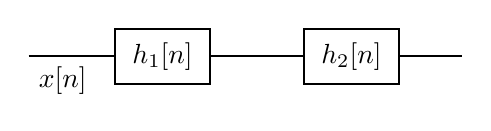
\begin{tikzpicture}[line width=0.7pt]
\node[draw,minimum width=1.2cm,minimum height=0.7cm] (a) at (0,0) {$h_1[n]$};
\node[draw,minimum width=1.2cm,minimum height=0.7cm] (b) at (2.4,0) {$h_2[n]$};
\draw (-1.7,0) node[below right]{$x[n]$} -- (a.west);
\draw (a.east) -- (b.west);
\draw (b.east) -- (3.8,0);
\end{tikzpicture}
\end{minipage}\hfill
\begin{minipage}[c]{0.56\linewidth}
\[
\begin{aligned}
\underline{\underline{y[n]}} &= \big(x[n]*h_1[n]\big)*h_2[n]\\
&= \underbrace{\big(x[n]*h_2[n]\big)}_{\color{morkalem}\hookrightarrow\ \delta[n]}*h_1[n]
\end{aligned}
\]
\end{minipage}

{\color{morkalem}\[ x[n]\,\delta[n-n_0] = x[n_0]\cdot\delta[n-n_0] \]}

\[
\begin{aligned}
\underline{x[n]}*\underline{h_2[n]} &= \big(\underline{\underline{\delta[n]}}-a\,\delta[n-1]\big)*{\color{morkalem}\boxed{\color{murekkep}a^n\cdot u[n]}}\\
&= a^n\cdot u[n] - \underbrace{a\cdot a^{n-1}}_{\color{morkalem}a^n}\cdot u[n-1] = a^n\underbrace{\big(u[n]-u[n-1]\big)}_{\color{morkalem}\delta[n]} = {\color{morkalem}\boxed{\color{murekkep}a^n}}\,\underset{\color{morkalem}n=0}{\delta[n]} = \underline{\underline{\delta[n]}}
\end{aligned}
\]

\[ \underline{\underline{y[n]}} = \underline{\delta[n]*h_1[n]} = \underline{h_1[n]} = \underline{\underline{\sin 8n}}\ \ \checkmark \]

\section{Ayrık zamanlı Fourier serisi}
\sayfa{19}
\begin{ornek}[(Soru)]
\textcolor{kirmizikalem}{Soru:} Aşağıda Fourier serisi katsayıları verilen $x[n]$ işaretini bulunuz.
\end{ornek}

\begin{center}
\begin{tikzpicture}
\begin{axis}[width=\linewidth,height=4.6cm,xmin=-14.5,xmax=17.5,ymin=-0.2,ymax=2.4,
  axis y line=none,xtick={-8,-4,-3,-2,-1,0,1,2,3,8},
  xticklabels={$-8$,\textcolor{kirmizikalem}{$-4$},\textcolor{kirmizikalem}{$-3$},\textcolor{kirmizikalem}{$-2$},\textcolor{kirmizikalem}{$-1$},\textcolor{kirmizikalem}{$0$},\textcolor{kirmizikalem}{$1$},\textcolor{kirmizikalem}{$2$},\textcolor{kirmizikalem}{$3$},$8$},
  xlabel={$k$},every axis plot post/.style={}]
\addplot[murekkep,ycomb,line width=0.9pt] coordinates {(-13,0.25) (-11,0.25) (-10,0.5) (-9,1) (-8,2) (-7,1) (-6,0.5) (-5,0.25) (-3,0.25) (-2,0.5) (-1,1) (0,2) (1,1) (2,0.5) (3,0.25) (5,0.25) (6,0.5) (7,1) (8,2) (9,1) (10,0.5) (11,0.25) (13,0.25) (14,0.5) (15,1) (16,2)};
\addplot[murekkep,only marks,mark=*,mark size=1.2pt] coordinates {(4,0)};
\node[above] at (axis cs:0,2) {\small $2$};
\node[above right] at (axis cs:1,1) {\small $1$};
\node[above right] at (axis cs:2,0.5) {\small $\tfrac{1}{2}$};
\node[above right] at (axis cs:3,0.25) {\small $\tfrac{1}{4}$};
\node at (axis cs:-14.2,0.15) {$\cdots$};
\node at (axis cs:16.9,0.6) {$\cdots$};
\node at (axis cs:16.8,2.1) {$a_k$};
\draw[kirmizikalem,->,line width=0.6pt] (axis cs:0,-0.62) -- (axis cs:0,-0.42);
\draw[kirmizikalem,->,line width=0.6pt] (axis cs:8,-0.62) -- (axis cs:8,-0.42);
\draw[kirmizikalem,line width=0.6pt] (axis cs:0,-0.62) -- node[below]{\small $N=8\,,\ T_0=8$} (axis cs:8,-0.62);
\end{axis}
\end{tikzpicture}
\end{center}

\vspace{4mm}
\noindent
\begin{minipage}[c]{0.42\linewidth}
\[ {\color{morkalem}\boxed{\color{murekkep}x[n] = \sum_{k=\langle N\rangle} a_k\, e^{-jk\omega_0 n}}}\footnotemark \]
\end{minipage}\hfill
\begin{minipage}[c]{0.55\linewidth}
\[ \omega_0 = 2\pi f_0 = \frac{2\pi}{N} \qquad {\color{kirmizikalem}\frac{2\pi}{T_0}} \]
\[ \omega_0 = \frac{2\pi}{8} = \frac{\pi}{4}\ \ {\color{morkalem}\checkmark} \]
\end{minipage}
\footnotetext{Claude notu: sentez denkleminde üs $+jk\omega_0 n$ olmalı; 20. sayfada pembe ile $+$ olarak düzeltilmiş.}

\[
\begin{aligned}
x[n] = \sum_{k=-4}^{4} a_k\cdot e^{jk\omega_0 n}
&= \underset{\color{kirmizikalem}\uparrow\ k=0}{\overset{\color{kirmizikalem}a_0}{2}}
+ \overset{\color{kirmizikalem}a_1=a_{-1}}{1}\cdot\underline{\Big[e^{-j\omega_0 n}+e^{j\omega_0 n}\Big]}
+ \overset{\color{kirmizikalem}a_2=a_{-2}}{\tfrac{1}{2}}\Big[e^{-j2\omega_0 n}+e^{j2\omega_0 n}\Big]\\
&\quad + \underset{\color{kirmizikalem}a_3=a_{-3}}{\tfrac{1}{4}}\Big[e^{-j3\omega_0 n}+e^{j3\omega_0 n}\Big]\\[2mm]
&= 2 + 2\cos(\omega_0 n) + \cos(2\omega_0 n) + \tfrac{1}{2}\cos(3\omega_0 n)\\
&= 2 + 2\cdot\cos\!\left(\frac{\pi n}{4}\right) + \cos\!\left(\frac{\pi n}{2}\right) + \frac{1}{2}\cos\!\left(\frac{3\pi n}{2}\right)
\end{aligned}
\]
\vspace{-2mm}
{\footnotesize\color{kursunkalem} Claude notu: son terimde $3\omega_0 = 3\pi/4$ olduğundan muhtemelen $\cos\!\left(\frac{3\pi n}{4}\right)$ olmalı.}

\noindent\sayfa{20}{\small\itshape\color{kursunkalem}(19. sayfanın pembe eklerle tekrarı: grafikte $k=4$'teki sıfır değerine ``4'' yazılmış; kutudaki ve açılımdaki üsler pembe $+$ ile düzeltilmiş; ilk köşeli parantezin altına $2\cos(\omega_0 n)$ yazılmış; $\tfrac{1}{2}\cos(3\omega_0 n)$ terimi okla gösterilmiş. Pembe ekler:)}

{\color{morkalem}
\[ x[n] = \sum_{k=\langle N\rangle} a_k\, e^{{\color{morkalem}+}jk\omega_0 n} \qquad\qquad
\underbrace{\Big[e^{-j\omega_0 n}+e^{j\omega_0 n}\Big]}_{2\cos(\omega_0 n)} \]
\[ \cos\theta = \frac{e^{j\theta}+e^{-j\theta}}{2} \qquad\qquad \sin\theta = \frac{e^{j\theta}-e^{-j\theta}}{2j} \]}

\[ {\color{morkalem}\checkmark\ \ \boxed{\color{murekkep} x[n] = 2 + 2\cdot\cos\!\left(\frac{\pi n}{4}\right) + \cos\!\left(\frac{\pi n}{2}\right) + \frac{1}{2}\cos\!\left(\frac{3\pi n}{2}\right)}} \]

\section{Sürekli zamanlı Fourier serisi}
\sayfa{21}
\begin{ornek}[(Soru)]
\textcolor{kirmizikalem}{Soru:} Aşağıda \okunamadi{verilen periyodik işaretin Fourier serisi açılımını bulunuz}.
\hfill{\small\itshape\color{kursunkalem}(satır ekran görüntüsünde kesik)}
\end{ornek}

\noindent
\begin{minipage}[c]{0.62\linewidth}
\centering
\begin{tikzpicture}
\begin{axis}[width=9cm,height=4.6cm,xmin=-3,xmax=5,ymin=-0.9,ymax=1.5,
  xtick={-2,-1,1,2,3,4},ytick={1},xlabel={$t$},ylabel={$x(t)$}]
\addplot[murekkep] coordinates {(-2,1) (-1,0)};
\addplot[murekkep] coordinates {(-1,1) (0,0)};
\addplot[murekkep] coordinates {(0,1) (1,0)};
\addplot[murekkep] coordinates {(1,1) (2,0)};
\addplot[murekkep] coordinates {(2,1) (3,0)};
\addplot[murekkep] coordinates {(3,1) (4,0)};
\addplot[kursunkalem,dotted,line width=0.6pt] coordinates {(-2,0) (-2,1)};
\addplot[kursunkalem,dotted,line width=0.6pt] coordinates {(-1,0) (-1,1)};
\addplot[kursunkalem,dotted,line width=0.6pt] coordinates {(1,0) (1,1)};
\addplot[kursunkalem,dotted,line width=0.6pt] coordinates {(2,0) (2,1)};
\addplot[kursunkalem,dotted,line width=0.6pt] coordinates {(3,0) (3,1)};
\addplot[kursunkalem,dotted,line width=0.6pt] coordinates {(-2.6,1) (4.4,1)};
\node at (axis cs:-2.6,0.55) {$\cdots$};
\node at (axis cs:4.6,0.8) {$\cdots$};
\fill[morkalem] (axis cs:1,0) circle (2pt);
\node[morkalem] at (axis cs:1.85,-0.65) {\small $(x_0,y_0)$};
\node[morkalem] at (axis cs:0.25,-0.65) {\small $(1,0)$};
\draw[morkalem,->,line width=0.5pt] (axis cs:0.45,-0.5) -- (axis cs:0.92,-0.08);
\draw[morkalem,->,line width=0.5pt] (axis cs:1.6,-0.5) -- (axis cs:1.08,-0.08);
\node[yesilkalem,above] at (axis cs:1.7,1.05) {\small slope $= \underline{\underline{-1}}$};
\end{axis}
\end{tikzpicture}
\end{minipage}\hfill
\begin{minipage}[c]{0.36\linewidth}
{\color{morkalem}\[ \boxed{\underset{\overset{\uparrow}{\text{slope}}}{m}\,(x-x_0) = y-y_0} \]}

\smallskip
{\color{yesilkalem}Doğru denk.:\ \ $\underline{(-1)}\cdot(x-1) = y \ \rightarrow\ \boxed{y = 1-x}$}
\end{minipage}

\vspace{1mm}
{\color{morkalem}\hrule height 0.8pt}
\vspace{2mm}

\[ \text{periyot:}\ \ \underline{\underline{T_0 = 1}} \ \ \rightarrow\ \ \omega_0 = \frac{2\pi}{T_0} = \underline{\underline{2\pi}}\ \ {\color{morkalem}\checkmark} \]

\noindent{\color{yesilkalem}Üstel seri Açılımı:\quad $\displaystyle x(t) = \sum_{k=-\infty}^{\infty} x_k\cdot e^{jk\omega_0 t}$}\ ,\qquad
{\color{morkalem}\boxed{\color{murekkep}\displaystyle x_k = \frac{1}{T_0}\int_{T_0} \underline{\underline{x(t)}}\cdot e^{-jk\omega_0 t}\,dt}}

\[ x_k = \int_0^1 (1-t)\cdot e^{-jk2\pi t}\,dt = \underbrace{\int_0^1 e^{-jk2\pi t}\,dt}_{\color{kirmizikalem}I_1} - \underbrace{\int_0^1 t\cdot e^{-jk2\pi t}\,dt}_{\color{kirmizikalem}I_2} = I_1 - I_2 \]

\[ I_1 = \int_0^1 e^{-jk2\pi t}\,dt = \frac{-1}{jk2\pi}\,e^{-jk2\pi t}\Big|_0^1 = \frac{-1}{jk2\pi}\Big[e^{-j2\pi k}-1\Big] = \frac{1}{j2\pi k}\left(1-e^{-j2\pi k}\right) \]

\noindent
$\displaystyle I_2 = \int_0^1 t\cdot e^{-jk2\pi t}\,dt$
\hfill {\color{kirmizikalem}Kısmi integrasyon:\ \ $\displaystyle\int u\,dv = u\cdot v - \int v\,du$}\hspace*{1cm}

\end{document}
